\documentclass[man, 12pt]{apa7} % 'man for manuscript, 12pt font size

\usepackage[american]{babel} % American English
\usepackage{csquotes} % Recommended with biblatex
\usepackage{pdflscape}

\usepackage{comment}

% Bibliography setup for APA style
\usepackage[style=apa, sortcites=true, sorting=nyt, backend=biber]{biblatex}
\addbibresource{mahbod.bib} % Your .bib file
\DeclareLanguageMapping{american}{american-apa}

% Additional useful packages
\usepackage{graphicx} % For including graphics
\usepackage{booktabs} % For professional quality tables
\usepackage{amsmath} % Enhanced math support
\usepackage{amsfonts} % Additional math fonts
\usepackage{amssymb} % Extended symbol collection
\usepackage{hyperref} % For hyperlinks in the document
\usepackage{pcl}
\usepackage{booktabs}
% Margins and spacing adjustments if needed
\usepackage{geometry}
\geometry{
    left=1in,
    right=1in,
    top=1in,
    bottom=1in
}
\usepackage{setspace}
\doublespacing % or \onehalfspacing

% Title, authors, and affiliations
\title{Individual Differences in Visual Illusions: Graphical and Analytic Approaches For Finding Structure in Real-World Cases}
\shorttitle{Individual Differences in Illusions}
\author{Mahbod Mehrvarz, Hrithik Popat, Jeffrey N. Rouder}
\affiliation{{University of California, Irvine}}


% Author note
\authornote{
   \addORCIDlink{MM}{0009-0002-5426-5867}
   
   \addORCIDlink{JNR}{0000-0003-2023-3891}

    Open Science Practices: The simulated data, analysis scripts, and code used to generate the figures are openly available at \href{https://github.com/specl/ind-illusions}{https://github.com/specl/ind-illusions}

   
   This research was supported in part by NSF 2126976 and by ONR N00014-23-1-2792.

   Correspondence concerning this article should be addressed to Mahbod Mehrvarz, Department of Cognitive Sciences, University of California, Irvine, CA, 92697. E-mail: mehrvarm@uci.edu
}



% Abstract and Keywords
\abstract{ 
    Are people who are susceptible to one illusion susceptible to others?  Previous research has shown small correlations, but might small values reflect attenuation from measurement error?  Data from 149 participants on 2 variants of 5 illusions were collected using an adjustment paradigm.  The resulting data are of notable high quality inasmuch as there is relatively little within-subject variability and relatively much between-subject variability ($\gamma^2 \approx 1.14$, reliability $\approx .93$).  Because the data are of such high quality, correlations may be estimated to high precision.  In line with previous research, these cross-illusion correlations are low in value, about .22$\pm .07$.  A Bayesian hierarchical analysis reveals that there is almost no attenuation from measurement error in these values.  Though correlations are low, latent variable analysis reveals that the pattern among these correlations yields a single, common latent factor. This factor loads on every illusion and accounts for about 25\% of the variance in each; thus it is a {\em susceptibility to illusions} factor.  We provide a novel set of statistical and graphical analyses focused on understanding the uncertainty in effects, correlations, and latent variables.}

\keywords{Individual Differences, Visual Illusions, Factor Analysis, Hierarchical Models, Reliability}


\begin{document}

\maketitle



Perceptual illusions have long been a topic of fascination to both the general public and scientists alike. The reason for this interest is straightforward: through the course of daily life, visual perception is primarily veridical and things, such as lines, typically appear as they are. Yet specific configurations can lead to distortion of our perception. An example of such a phenomenon is the Brentano illusion, depicted in the first row of Figure~\ref{fig:illPlots}. While the blue and the red lines are the same length, depending on the orientation of the arrowheads, one appears longer than the other. 

For scientists, perceptual illusions offer a window into the processes and mechanisms underlying perception \parencite[]{Coren.Girgus.2020}. Recently, individual differences have been focal \parencite[see][]{Tulver.2019}. The central query concerns correlations in the magnitude of illusions across individuals: are people who are particularly susceptible to one illusion also more or less susceptible to other illusions? The more refined question concerns the pattern of correlations across a collection of visual illusions.  Specific patterns may indicate factors or clusters.  For instance, perhaps size-constancy illusions cluster together but are independent of illusions based on the misattribution of 3-D structure. It is in this way that the factor structure of individual differences offers insight into the underlying processes and mechanisms. 

Research exploring individual differences in susceptibility to illusions is precedented. Most studies report no common mechanism underlying perceptual illusions \parencite[]{Mazuz.etal.2023, Grzeczkowski.etal.2017, Cretenoud.etal.2019, Bosten.etal.2017, Cottier.etal.2023, Ward.etal.2017}. These studies often found significant correlations within variants of specific illusions, but they only found weak correlations between different types of illusions (with few exceptions).  The resulting conclusion is that factors influencing susceptibility to illusions are likely multiple and specific rather than singular or general.  These results concord well with a lack of general factors in visual perception studies, where a prevailing explanation is that individual variation likely reflects uncorrelated biological aspects such as retinal structure \parencite[e.g.,][]{Mollon.etal.2017, Bosten.Mollon.2010}. Conversely, general factors are prevalent in studies of cognition, as seen in areas such as intelligence \parencite[]{Jensen.1998} personality \parencite[]{OConnor.Paunonen.2007}. In fact, cognitive abilities often yield positive correlations, a concept known as Spearman's positive manifold \parencite{Ritchie.2015}. In keeping with the trend found in studies of cognition, \textcite{Makowski.etal.2023} have indeed found a general factor underlying perceptual illusion. Moreover, they claim this general susceptibility factor is positively related to positive personality traits (such as agreeableness) and negatively related to dark-triad personality traits. 

Conflicting results and the inability to identify common mechanisms with individual differences are not unique to visual illusions.  Perhaps the best-studied domain for individual differences in experimental setups is cognitive control \parencite[]{Enkavi.etal.2019, Rey-Mermet.etal.2019, Draheim.etal.2019}.  The results in this domain have been underwhelming, characterized by low correlation among tasks that purportedly measure the same construct and unstable latent decomposition \parencite{Karr.etal.2018}.  Indeed, the results in cognitive control and visual illusions are similar in that correlations are low, and latent decompositions are likely unstable.  This may not be a coincidence---it may reflect how we as a field tend to analyze data. 

One pervasive problem in the study of individual differences in experimental contexts is assessing uncertainty.  The main statistic, the correlation coefficient, has a difficult property in these studies: it is not \textit{consistent}.  Consistency refers to a long-run property, a statistic is consistent if, with enough data, it converges to the true value of what it is supposed to measure.  The sample mean, for example, is consistent.  As the number of samples increases, it is guaranteed to converge to the true or population mean, and moreover, for any sample size, we can assess how much uncertainty there is in our knowledge of this true value. Sample correlations, in contrast, do not converge to the true population value unless each individual's score is measured without error.  When there is error, termed \textit{measurement error}, then it is well known that sample correlations converge to a value that is lower in magnitude than the true value.  The statistical phenomenon is termed \textit{attenuation from measurement error}, and it has been known for over 100 years \parencite[]{Galton.1888, Spearman.1904}. When there is much measurement error, as there is in many experimental contexts, observed correlations are artifactually small and latent variable analyses are unstable \parencite[]{Rouder.etal.2024, Hedge.etal.2018, Karr.etal.2018}.

There is a silver lining in this otherwise difficult state of affairs reflecting the specific nature of experiments.  In experiments, participants often perform many repeated trials per condition per task.  In the usual course of analysis, the variability here is ignored.  Researchers compute a single summary score per person per task, and the matrix of these person-by-task scores serves as input for describing the correlations among tasks or performing further latent variable analysis.  Yet, it is crucial to understand trial-by-trial variability as it forms the basis for understanding the uncertainty in the data.  We leverage modern trends in modeling and estimation to keep a focus on uncertainty.


We have two goals of equal weight in this report.  First, we study the nature of individual differences in visual illusions with a focus toward understanding the amount of covariation between illusions and the underlying factor structure.  Second, we analyze the data with a focus toward characterizing the uncertainty in data by consideration of multiple sources of variability.  This second aspect is both modern and novel, and we think our analyses serve as a blueprint for enhancing the understanding of variability and uncertainty of individual differences in experiments.

To study individual differences in illusions, we constructed a battery of tasks. In each task, the participant had to adjust an object so that it matched another part of the display.  For example, in the Brentano Illusion, participants adjusted the middle chevron until the size of the blue and red segments appeared equal in length.  We build a pipeline in the analysis section.  To preview, much effort is spent graphically examining how well we could measure each person's bias or score on each task.  It is only after demonstrating that people differ and that we could reliably measure these differences that we perform a latent-variable decomposition of the correlations among the tasks.  To foreshadow, we find a middle position inline with most of the previous research.  First, correlations are small, and this small size is not due to attenuation or statistical issues.  Individual differences in various visual illusions are large, but the correlations across different illusions are truly small.  Second, even though these correlations are small, we know them with relatively high precision, and they form a positive manifold. There is a common factor---susceptibility to illusions.  Unfortunately, it accounts for just a small fraction of the variance.  Much of the variability therefore seems to be idiosyncratic to specific illusions.

\section{Method}

The experiment was run under UCI IRB \#3292. A demonstration version with all the tasks may be found at \href{https://specl.socsci.uci.edu/acquire/data4/iBat5/demo.html}{https://specl.socsci.uci.edu/acquire/data4/iBat5/demo.html}.

\subsection{Participants}

150 individuals, recruited through Prolific, served as participants in the experiment. The only constraint was that participants were located in the United States.  Participants were paid  \$5 USD for the 20 minutes it took to complete the battery.


\subsection{Tasks} 

The task battery comprises five visual illusions: the Brentano Illusion \parencite{Brentano.1892}, the Ebbinghaus Illusion \parencite[]{Ebbinghaus.1913}, the Poggendorff Illusion \parencite[]{Day.Dickinson.1976}, the Ponzo Illusion \parencite[]{Ponzo.1910}, and the Zöllner Illusion \parencite[]{Judd.Courten.1905}. These illusions are shown in Figure~\ref{fig:illPlots}. In each task, participants adjusted a critical element of the stimulus. In the Brentano illusion (Panels A), participants adjusted the middle chevron to make the blue and red lines appear to be of equal length, with a tendency to set the red line too long and the blue line too short. In the Ebbinghaus Illusion (Panel C), participants adjusted one of the inner circles to match the other in size. In the Poggendorff Illusion (Panel D), participants aligned one of the two disjointed segments (left and right levers) to form a straight line. In the Ponzo Illusion (Panel E), participants adjusted one of the red lines to align with the other line. Lastly, in the Zöllner Illusion (Panel F), participants adjusted the horizontal lines to appear parallel. The method of adjustment was employed as it is long-standing \parencite{Fechner.1860} and effective in measuring the strength of illusions \parencite[]{Cretenoud.etal.2021}.

For each task, we constructed two versions. The two versions of the Brentano Illusion are shown in Panels A and B. The motivation for using two versions is to control for idiosyncratic response biases. If a participant ran only the version in Panel A and had a natural tendency to set the left segment too large at the expense of the right segment, this tendency would manifest as a larger illusion effect. To control for such a possibility, no matter how remote, we constructed an alternate version so that such a tendency would not greatly impact the true illusion effect. Alternate versions of each illusion were constructed analogously. For the Ebbinghaus Illusion, in Version 1, participants adjusted the right inner circle (surrounded by smaller circles); in Version 2, they adjusted the left circle (surrounded by larger circles). For the Poggendorff Illusion, in Version 1, participants adjusted the right lever vertically. In Version 2, the illusion was flipped vertically, with the downward-facing right lever being adjusted on the right-hand side. For the Ponzo Illusion, in Version 1, participants adjusted the closer red line, and in Version 2, they adjusted the farther red line. Lastly, Zöllner Version 1 is depicted in Panel F of Figure~\ref{fig:illPlots}, and Version 2 was the same but mirrored horizontally. We expected the magnitude of an illusion for an individual to be consistent across versions. This expectation held for some illusions, but surprisingly, not for others. As such, we could not collapse across the versions and they feature prominently in the subsequent analyses.


\subsection{Design}

The design was a $5 \times 2$ within-subject factorial design. The first factor was the task (the specific illusion), and the second factor was the task version.  We chose to repeat each task-by-version combination 15 times for each individual.  This trial size of 15 was chosen as follows.  We ran a pilot experiment to assess the size of illusions, the variability between people, and the variation across replicate trials.  We then used the method described in \textcite{Rouder.Mehrvarz.2024} to obtain an expected reliability of over .95 per illusion.  The method yielded 30 trials for each illusion which we split across versions.  The response measure was how far the adjustment varied from the ground truth.

\subsection{Procedure}

Participants registered through Prolific, and were then referred to our webserver for the experiment. After reading the consent letter, they were asked to raise the volume on their speakers so they could hear feedback tones and to size their screen so that they could see all stimulus elements.  Participants ran two cycles, and in each cycle, each of the five illusions was presented in a random order. Versions were randomly chosen in the first cycle, and the other version was presented in the second cycle. For each illusion in the cycle, a set of instructions and two practice trials were provided, and then the participant ran 15 replicate trials. Across all tasks and cycles, there were 150 trials in total. Participants had to adjust elements as discussed previously using the arrow keys on their keyboard, and each press moved the critical element a small amount. When they were satisfied with their adjustment, they pressed the spacebar, which advanced to the next trial. Breaks were given after tasks of 15 trials.


We found in a pilot that participants varied greatly in how much time they took before being satisfied with their adjustment. Some would spend tens of seconds going back and forth until they made the spacebar commitment. To keep the experiment fairly regular across individuals, it was necessary to impose an eight-second time limit. Participants could advance to the next trial by pressing the spacebar or wait the eight seconds for automatic advancement.


For each trial in each illusion, we varied a number of parameters. For convenience, several illusions have a \textit{target} size, such as the size of the to-be-matched line segment (Brentano, Ponzo), circumference (Ebbinghaus), or position (Poggendorff). We jittered these target sizes as well as the starting sizes of the adjusted elements. We also jittered other elements, including the overall position on the screen and, in the Zöllner illusion, the length of the main lines and cross lines. This variation prevented the development of stereotypical responses across repeated trials.


\section{Analysis}

On each trial, participants produce an adjustment that may differ from the ground truth. We scored the illusion effect as follows: For the Brentano Illusion, the score was the number of pixels to the left (or right) of half of the horizontal segment relative to the size (in pixels) of the segment. The mean effect, in this case, was 6.6\%, and this sized effect is indicated in Figure~\ref{fig:effectPlots}. Relative effects were used for the Ebbinghaus and Ponzo illusions, each was the difference between the adjusted value and the true value relative to the size of the true value. For the Poggendorff and Zöllner illusions, however, there is nothing to compare the adjustments against. Therefore, the scores were measured as the number of displaced pixels (Poggendorff) or the angle from horizontal (Zöllner).


\subsection{Data Cleaning}

The adjustment paradigm here consisted of making several keypresses to finely adjust objects. This process takes longer than conventional response times, and typical responses are in the 5-second range. We were concerned about participants who sped through their judgments to complete the task quickly. When we plotted the histograms of response times, there was a separate mode below 600 ms. This mode was not large, and overall, only 1.5\% of responses fell here. These responses were excluded, as were individuals who had more than 5\% of their responses in this mode (5 individuals). Next, we conducted a univariate analysis to detect outliers based on standardized scores across different tasks and their respective versions. Participants whose z-score on any task exceeded 4 were removed (6 individuals). A participant inadvertently completed the experiment twice, and therefore their second attempt was excluded. A document detailing the data-cleaning process and the corresponding code can be found on the project's GitHub repository.


\subsection{Tasks In Isolation}

The goal of the analysis is to understand the relationships among the tasks. However, tasks must be suitable in that they measure a signal without an undue degree of noise. If individual task scores are too noisy, then correlations are attenuated too low, and latent-variable decompositions may be unstable \parencite[]{Rouder.etal.2023}. The first step, then, is to provide a deep dive into the noise in task scores themselves. We do so before considering the relationships among tasks.

{\bf Size of the effects.}  The issue of the size of effects in individual-difference studies is often secondary. Here, the effect refers to the size of an illusion; in cognitive control tasks, the effect might be the slowing in an incongruent condition relative to a congruent one. When individual-difference studies are conducted, the focus is on covariation and correlation, and the size of the effect, such as the mean difference in response times across conditions, does not enter into the critical parts of the analyses. Yet, the effect sizes may serve as an indicator of the robustness of subsequent individual-difference analyses. When effects are large, there is substantial headroom for people to vary. When effects are small, there is far less headroom. A good first check, then, is the size of the effect.


We computed an effect size and a $t$-value for every individual in each of the 10 tasks.\footnote{Effect size for the $i$th individual in the $j$th task is $d_{ij}=m_{ij}/s_{ij}$, where $m_{ij}$ and $s_{ij}$ are respectively the sample mean and sample standard deviation for all trials for the $i$th individual in the $j$th task.  The $t$-value is $t_{ij}=d_{ij}\times\sqrt{K_{ij}}$}  Figure~\ref{fig:effectPlots}A shows a histogram of all effect sizes and $t$-values, and they are nothing short of spectacular in value.  Even though there are at most 15 trials per individual per task version, the vast majority of the effect sizes exceed Cohen's .8 criteria for large, and even more are significant at .05 level.  Figure~\ref{fig:effectPlots}B shows these effects tabulated by task as empirical cumulative distribution functions.  Even though there are differences across the tasks in mean effect sizes and the spread of effect sizes, the large effect sizes hold for all 10 tasks.  In summary, visual illusions are so large that performance from just 15 trials contains a larger signal than typical cognitive studies comprised of thousands or tens-of-thousands of trials!     

{\bf Discriminating among individuals within a task.}  For the remainder of the analyses, we used scaled scores as follows.  For each task, MSE was computed among individuals, and the square-root is the standard deviation of task-specific residual variance.  Then, each score for all individuals in a task was expressed in units of this standard deviation, that is, in task-specific effect size units.\footnote{Let $Y_{ijk}$ be the $k$th replicate observation for the $i$th person on the $j$th task.  Let $s_j=\sqrt{\mbox{MSE}_j}=\left(\sum_{ik}(Y_{ijk}-m_{ij})^2/I(K-1)\right)^{1/2}$. Then the task-scaled score is $Y_{ijk}/s_j$.}  Figure~\ref{fig:taskPlots} shows these scaled scores in a configuration that we term {\em task plots}.  Here, individuals' mean scaled scores in each task are ordered and plotted with 95\% confidence intervals.  We see here that there are substantial differences in scores in all tasks across individuals indicating that we can well localize individual effects and well discriminate among individuals.  We recommend that task plots always be included.  In many ways, they tell what is possible.

{\bf Goodness of Task Measures.}  The usual way to understand the goodness of a task is reliability.\footnote{One course is to split the trials, compute the correlation, and scale it up to the full sample size through the Brown-Spearman prophecy formula.  This is a test-theory approach that fails to leverage the fact that experiments are comprised of multiple replicate trials.  Reliability here is computed directly from within-trial and across-trial variabilities, see \textcite{Rouder.Mehrvarz.2024}}.    There is, of course, a direct relationship.  The larger the spread of the mean scores relative to CIs in the task plots in Figure \ref{fig:taskPlots}, the higher the reliability.  Yet, both task plots and the associated reliability measure strike us as incomplete for communication about tasks.  

This incompleteness comes from the fact that reliability and task plots are tied intimately to the number of replicate trials.  The Stroop task, for example, is unreliable with 15 trials, but it is very reliable with several thousand trials \parencite[]{Lee.etal.2023}.  What is needed for grounded communication is a task measure of signal-to-noise that does not depend on the number of replicate trials.  We advocate the signal-to-noise ratio of a task as such a measure \parencite[]{Rouder.Mehrvarz.2024}, and denote it as $\gamma^2$.  The signal, the numerator of $\gamma^2$, is the variability across individuals' true scores in a task.  The noise, the denominator of $\gamma^2$, is the trial-to-trial variability.  Tasks with high values of $\gamma^2$ are reliable even with few replicate trials per individual per task; tasks with low values are reliable only if there are a high number of replicate trials per individual per task.  The $\gamma^2$ for each illusion is denoted in the task plot, and the average is 1.145.  This value means that across illusions, variation across people is almost as big as variation within a trial.  It is a large value by any standard, and it should be possible to understand individual differences to high precision.

{\bf Split-Half Reliability: A Sanity Check.}  In the preceding plots, we showed that the illusion effects are quite large and that individuals can be discriminated.  We provide one final check on this sanguine state---a split-halves scatter plot.  Plotted are individual mean effects for the second-half of trials as a function of the mean effects for the first-half of trials (Figure~\ref{fig:relPlots}).  As can be seen, the association---the split half reliability---is quite high.  

In summary, with such large and reliable effects, it should be straightforward to assess the relations among tasks without excessive variability or attenuation.

\subsection{Relations Among Tasks}

Now that we have established that these tasks have very high signal-to-noise characteristics, the next step is analyzing the relations among them.  Figure~\ref{fig:corPlot} shows the correlations among the tasks obtained in two different ways.  The upper triangle shows the conventional sample correlations; the lower triangle shows estimates from a hierarchical Wishart model that disattenuates these correlations for trial noise.  The hierarchical Wishart model is from \textcite{Rouder.etal.2023}, and it is comprised of two levels: a data level and an individual-effects level.  At the data level, it is assumed that performance on a trial results is the sum of a individual-by-task true score and trial noise.  Let $\theta_{ij}$ denote this true score for the $i$th individual on the $j$th task, and let $\bftheta_i=(\theta_{i1},\ldots,\theta_{iJ})$ denote the vector of true task scores for the $i$th individual.  At the individual-effect level, a multivariate random effects model is placed of $\bftheta_i$: $\bftheta_i \sim \mbox{Normal}_J(\bfmu,\bfSigma)$.  The key here is that all relations among the tasks are in the variance $\bfSigma$.  We estimate $\bfSigma$ in the Bayesian framework, and as such, a prior is needed.  The Wishart prior \parencite[]{Wishart.1928} serves as practical choice as it places little \textit{a priori} constraint on $\bfSigma$ while insuring that posterior values for a valid variance matrix (that is, they are symmetric and positive-definite matrices).  The advantage of the Bayesian framework is two-fold.  First, it is conceptually straightforward approach for separating trial noise from across-individual variation.  Second, analysis is computationally convenient with modern MCMC sampling methods \parencite[]{Gelfand.Smith.1990}.  Posterior of correlations, derived form the variance matrix, are be computed within each iteration of the MCMC chains.  The posterior mean is shown in the lower triangle of Figure~\ref{fig:corPlot}.

Comparisons of the sample correlations and model-based correlations reveal a tight correspondence indicating little attenuation in sample correlations.  This lack of attenuation is relatively rare in experimental settings and reflects that effects are large relative to trial noise.  First, the within-version correlations.  For three illusions, the Ponzo, Poggendorf, and Zoellner, there are high correlations across the two versions of the illusions; for the other two illusions, the Brentano and Ebbinghaus, the correlations are more modest.  This result is surprising.   We had expected high correlations, and the task versions were included as a control for response biases.  The modest correlations indicate that it is not wise to average scores across versions.  Second, the cross-illusion correlations.  Each of these is positive in direction and modest in value.  We examine these values in the context of uncertainty.

{\bf Uncertainty In Correlations.}  We recommend that researchers study the uncertainty in cross-task correlations.  In designs where participants provide repeated trials per task score, there are two sources of uncertainty.  One is from the noise across trials.  The degree of uncertainty from this source reflects not on the degree of trial-to-trial variation, but the number of trials in each cell.  The more trials, the less influence this variation has on the uncertainty of the correlation coefficient.  The other source reflects variation across individuals, and the more individuals the less uncertainty from this source. These sources may be combined into an overall assessment with the hierarchical Wishart model.  The 95\% posterior credible interval (CIs) serves as a suitable measure of uncertainty.  

Figure~\ref{fig:ciCorPlots} shows the mean and uncertainties (95\% CIs) for the correlations.  Consideration of them provides the following insights:  First, as noted, many of them are undoubtedly positive providing evidence for a positive manifold across illusions.  Accordingly, there is at least one factor in common.  Second, the three highest correlations, which stand apart, are correlations among different versions of the tasks.  If we focus on correlations across different illusions, there is not so much variability.  These are clustered around .22 in value with credible intervals that have a full width of .134 ($\pm .067$) on average.  This small value, .22, is by-and-large confirmation of previous results.  One visual illusion accounts for about 4.7\% of the variance in another illusion. 

\subsection{Latent Variable Analyses}

Interpreting sample correlation such as those in Figure \ref{fig:corPlot} is often aided by latent-variable models.   Latent variable modeling, unfortunately, is a bit of a dark art in our view.  While implementation and analysis is relatively straightforward in modern packages, making judicious choices in specification and providing sound interpretation is challenging \parencite[]{Preacher.MacCallum.2003, Armstrong.1967}.  In visual perception, \textcite{Tulver.2019} recently notes that many of these issues, what is a factor, how to measure factors, and how to interpret factors, remain unresolved in the field.  Here, even though the data are of high quality, we run head-long into these difficulties. 



\textbf{Principle Components.}  Many researchers who search for factor structure use principle component analysis (PCA).   Table~\ref{tab:EFA-10} shows the eigenvalues accounted for by each component. Accordingly, there are four factors with eigenvalues greater than 1.0. 

PCA is often seen as interchangeable with factor analysis.  Though similar, there are critical differences.  For experimental psychological research, the latter is superior to the former.  To see the key difference, consider the test case where there is no structure---that is, the correlation matrix is a diagonal matrix plus a small random variation from trial noise.  The PCA for $J$ tasks would yield $J$ factors each accounting for about $1/J$ proportion of the variance.   The factor model underlying factor analysis, however, has error terms that account for uncorrelated noise.  For the test case, the residuals from these error terms would be large, and the factor loadings on illusions that account for the structure would be quite small.  This difference has been well known \parencite[]{Velicer.Jackson.1990} and goes under the moniker that factor analysis partitions common variance rather than total variance \parencite[]{Kline.2023}.  Because factor models are much easier to interpret in low-signal scenarios, they should be used instead of PCA in vision, cognitive control, and related fields.

{\bf Exploratory Factor Analysis.}  We performed exploratory factor analysis (EFA) separately for 1 to 6 factors.  Table~\ref{tab:EFA-10} also shows the model selection statistics, and as can be seen, the situation is ambiguous.  While inspection of eigenvalues (first column) indicates support for a one-factor or four-factor solution, AIC indicates a five-factor solution and BIC indicates a three-factor solution.  Examination of the varimax factor loadings for 5 factors is shown in Table \ref{tab:Fac-10}. Factors tend to load on a single task with only modest cross-task loading.  With this result, as well as the ambiguity of dimensions, it is difficult to gain much additional insight above that from the sample correlations.  

{\bf Confirmatory Factor Analysis.} We also performed a series of confirmatory factor analyses with models shown in Figure~\ref{fig:cfa}.  In the models in Figure~\ref{fig:cfa}A-B, the manifest versions of each illusion load onto a latent variable.  Correlations across the five latent variables are then computed (Fig~\ref{fig:cfa}A) or modeled with additional latent factors (Fig~\ref{fig:cfa}B).  The main problem we encountered was that the resulting parameters had substantial negative variance components rendering them inadmissible. The problem is a Heyward Condition problem \parencite[]{Rindskopf.1984}, and it occurs because the Brentano Illusion has low version correlations:  for example Version I of the Brentano Illusion is better predicted by the Zöllner Illusion than by Version II of the Brentano Illusion.  We also tried a more flexible version, Figure~\ref{fig:cfa}C), but encountered the same issues.


{\bf Removing Version Correlations.}  It is now clear that the preceding latent variable analysis was influenced by the three high within-task correlations.  We wondered if it is possible to find structure above and beyond within-version correlations  One approach is to use confirmatory factor models where there are dedicated factors for versions.  Then additional exploratory factors could be included.  Such a model can indeed be analyzed in Lavaan, yet, at least in our hands, we were unable to find suitable solutions where variances were unanimously positive.

A far simpler approach is using one version of each task.  We picked the version of each task that had the best signal-to-noise ratio $\gamma^2$.  These five versions, one for each task, were entered into an exploratory factor analysis.  The results (shown in Table~\ref{tab:EFA-5} were that a one-factor model was superior to a two-factor model by AIC and BIC (3.0 and 14.4 points, respectively), and CFI (.989) and $\chi^2$ values ($p\approx .35$) indicates no detection of misfit.  The loadings and variabilities associated with this one-factor solution are given in Table~\ref{tab:Fac-5}.  

In latent variable modeling, it is desirable to assess how much of the variance is accounted for and how much of what remains is residual.  The variability accounted is obtained by adding commonalities (or taking the trace of the loading matrix), the variability residuals are explicit parameters.  For this one-factor model, the single-factor structure accounts for about 24.7\% of the variance, which is substantially higher than the 5\% from squaring correlations.  In the discussion, we discuss why these differences occur and how to interpret them in drawing scientific conclusions.



\section{Discussion}

In this paper, we paid equal attention to the substantive issue of how visual illusions covary across individuals and the methodological issue of how to document structure in this covariation.  The following conclusions may be drawn substantively about visual illusions:  

1. Visual illusions are strikingly large in effect and straightforward to document.  Data from each of our participants in each task, comprising at most 15 observations, often shows more evidence of an effect than typical cognitive psychology experiments comprised of hundreds of observations from scores of participants.  

2.  Individual differences are large.  The amount of variance across individuals is large relative to trial noise.  The ratio is around 1.145-to-1 (in variances), which is about 73 times larger than those in cognitive control tasks \parencite[]{Rouder.etal.2024}.  

3. Correlations across different illusions are relatively small.  This small size is not due to statistical attenuation but reflects the true state of things---illusions are at most weakly related.  

4. Nonetheless, there is at least one common factor, moreover, this factor accounts for 24.7\% of the total variance.

Our methodology for uncovering the structure of individual differences has a few elements that are not commonly stressed: 

1. We spend much effort assessing how much individual variation is recoverable.  The task plots in Figure~\ref{fig:taskPlots} show how different individuals are in each effect.  If these differences are hard to discern graphically, then it may be hard to document correlations among tasks.

2. Understanding the uncertainty in correlations is key to placing them in context and performing subsequent latent-variable modeling.  The plot in Figure \ref{fig:ciCorPlots} shows immediately that with the exclusion of version correlations, correlations are modest and fairly uniform, and moreover, there is a positive manifold across them.   The modesty of these correlations relative to uncertainty means that it is not possible to derive a many-factor solution.  One issue is that obtaining these uncertainties is not straightforward.  They come from a hierarchical model where the data model accounts for trial-to-trial variation and the model of individuals accounts for between-participant covariation.  Bayesian hierarchical models are perfect for this endeavor and there are a wide range of successful applications and tutorials for psychologists. 

3. Latent-variable modeling was difficult on several accounts.  The main problem was accounting for high version correlations for some illusions while accounting for lower version correlations in others.  We relied on the inspection of the correlations for guidance.

\subsection{Interpretation}

In the literature, there are seemingly two incompatible results.  The first is that individual differences in visual illusions are at best weakly correlated \parencite{Cretenoud.etal.2019} and the proportion of variance accounted for any illusion on any other is surprisingly small.  The second is that individual differences are related by a common factor which may even reflect personality differences \parencite[]{Makowski.etal.2023}.  We find support for both positions.  Visual illusions are undoubtedly weakly related.   Individual differences in any one illusion account for 4.7\% of the variance in another.   And, visual illusions are connected by a common factor that accounts for 24.7\% of the variance in each illusion when one version of each is entered into the analysis.  Of course, both proportions of variance are correct---this is how latent variables work.  One task may explain $a_1$ of the variation in the latent variable; the latent-variable may explain $a_2$ of the variation in another task, and, assuming these proportions are independent, then the first task explains $a_1\times a_2$ of the variance in the second.

In the introduction of this paper, we raised the hope that patterns of individual differences could inform about the structure of perception and cognition that underlie these illusions.  That hope remains unrealized.  There most definitely is common variation, but it seems too small to finely decompose, and, consequently, too small to understand the perceptual and cognitive factors that mediate illusions.  Moreover, because this variation is small and loads on all tasks, it may have little to do with illusions per se.  An alternative is that the factor relates to how people engage in computer tasks or how conscientious they are \parencite{Makowski.etal.2023}.  


\subsection{Future Directions}

The set of results that strikes us the most as cognitive psychologists is comprised of version correlations.  For some illusions, a small change in setup designed to reverse the direction of the illusion does exactly this.  Consider the Zöllner illusion.  In Figure 1F, the top horizontal line appears slanted such that the left end is higher than the right end.  In the alternative version (not shown), the cross lines are rotated 90 degrees.  The bias reverses as expected---the top horizontal line appears slanted such that the left end is lower than the right end.  And, the correlation is high---people who show larger biases in one version show large reverse biases in the other.  This reasonable expectation does not hold for the Brentano or the Ebbinghaus Illusions.  For instance, in the Brentano illusion (Figure 1A), people set the chevron too far to the left.  In the alternative version (Figure 1B), they set it too far to the right.  These biases correlate moderately with other illusions, such as the Zöllner and Poggendorf.  Yet, the two versions have surprisingly little correlation between themselves.  Neither of these results is a statistical fluke as the data are highly reliable and the 95\% credible intervals on the correlation coefficients are well separated (see Figure~\ref{fig:ciCorPlots}).  How is this pattern so?  What about the Brentano and Ebbinghaus Illusions make them pathological in this regard?  Perhaps, rather than clustering illusions based on how well they correlate to each other, we should study how well they correlate within themselves, that is, how robust they are to reasonable configurable changes.  It may be this robustness that provides insight into the mechanisms after all.

One inelegant piece in this report is the lack of articulation between the model of uncertainty (the hierarchical Wishart) and the factor models (implemented in \texttt{Lavaan}).  We worried little about this because the data are highly reliable, and the sample correlations are close to model correlations.  Yet, for other applications, it would be desirable to have an integrated modeling solution where data components that describe trial-to-trial variability are coupled with latent variable models of individual differences.  In these models, uncertainty reflects contributions from variability at the trial level and from the individual-difference level.  

As a field, we are near this goal.  \textcite{Merkle.etal.2021} provides \texttt{blavaan}, which is an \texttt{R} package for factor analysis.  The advantage here is that `blavaan` will output code that runs in \texttt{stan} \parencite[]{Carpenter.etal.2017} or \texttt{JAGS} \parencite[]{Plummer.2003}.  It seems plausible that these outputs may be modified for hierarchical settings to include trial-level model components.  Another example comes from  \textcite{Stevenson.etal.2024} who has very recently developed an integration model.  The data model is a drift-diffusion data model that accounts for trial-to-trial variability; the prior on drift rates is a factor model that accounts for individual differences.  We have integrated the two components in \textcite{Mehrvarz.Rouder.2024}, but the focus is on estimating correlations accurately without assessment of factor structures.  Given these exciting developments, it may not be long until experimental psychologists have straightforward tools to routinely perform trial-noise integrated factor analysis. 


\printbibliography

\begin{figure}
    \centering  % Centers the figure
    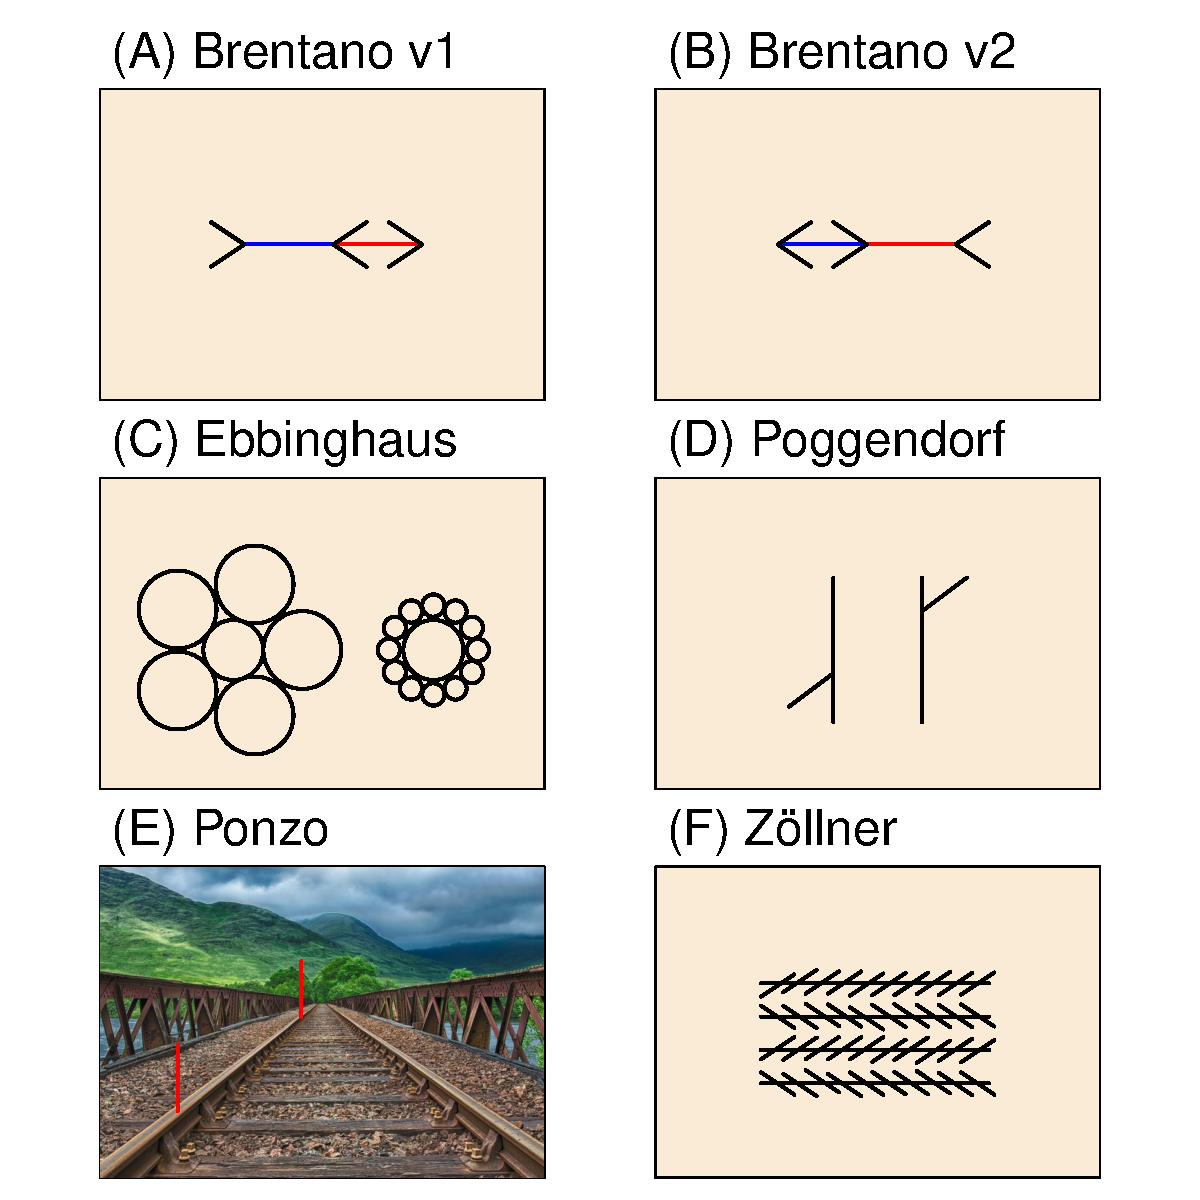
\includegraphics[width=6.5in, height=6.5in]{_figs/ill-tasks.pdf}
    \caption{{\bf Illusion Tasks:} A-B. Two versions of the Brentano Illusion were presented. Participants adjusted the center chevron so that the red and blue lines appeared equal in length. C. In the Ebbinghaus Illusion, participants adjusted the right inner circle in Version 1, while in Version 2, they adjusted the left inner circle. D. For the Poggendorf Illusion, participants adjusted the right lever vertically in Version 1. In Version 2, the illusion was flipped vertically, with the downward-facing right lever being adjusted on the right-hand side. E. In the Ponzo Illusion, participants adjusted the closer red line in Version 1 and the farther red line in Version 2. F. For the Zöllner Illusion, participants adjusted the horizontal lines to appear parallel. Version 1 is depicted in the figure and Version 2 was exactly the same but mirrored horizontally.}
    \label{fig:illPlots}
\end{figure}


\begin{figure}
    \centering  % Centers the figure
    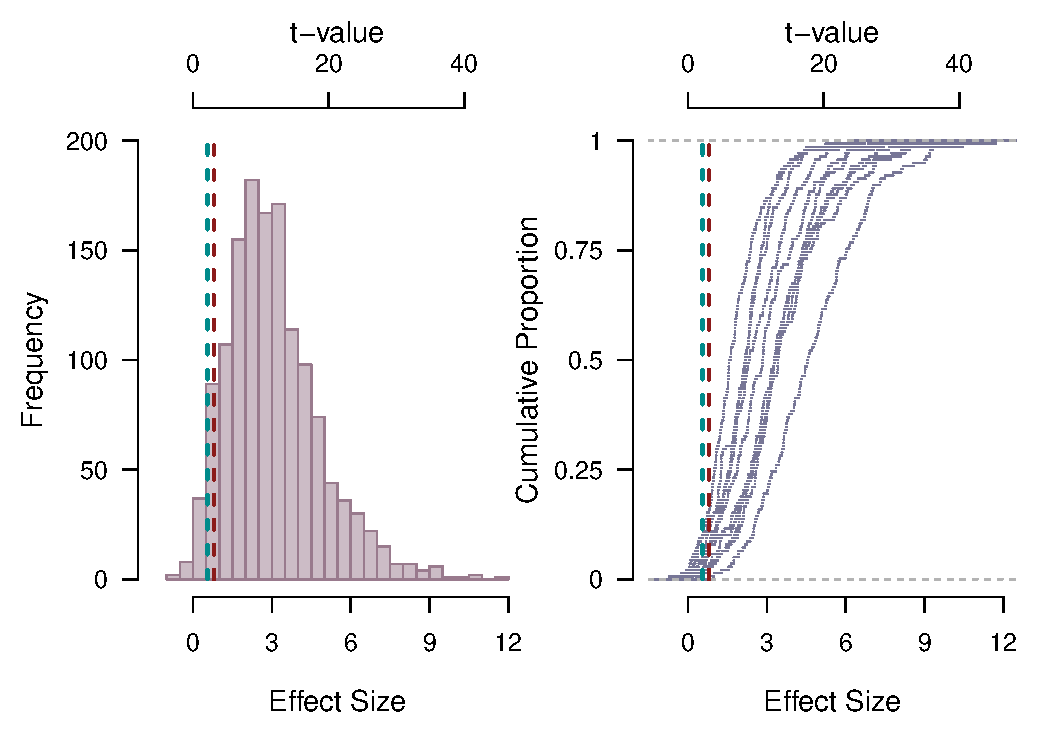
\includegraphics[width=6in, height=5in]{_figs/effect-plot.pdf}
    \caption{The size of illusions effects. The data from each participant in each task is treated as a separate experiment. Left: Histogram of all effect sizes shows large effects for almost all combinations of individuals and tasks.  Right: The same data plotted as an empirical-cumulative-distribution function reveals although there are large effects for all tasks, there are some differences across the tasks.}
    \label{fig:effectPlots}
\end{figure}

\begin{figure}
    \centering  % Centers the figure
    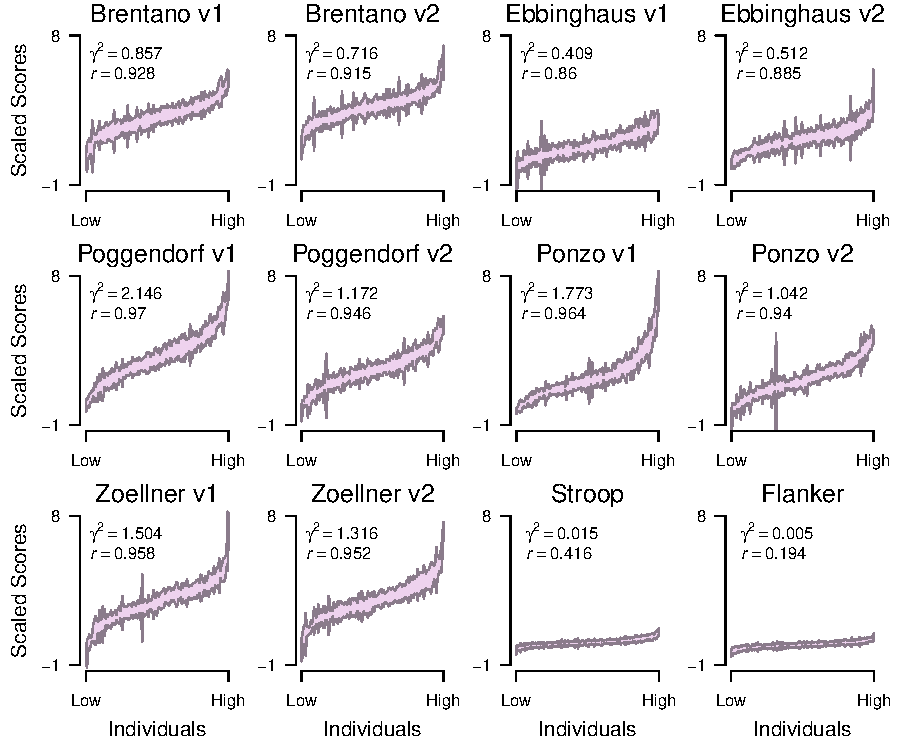
\includegraphics[width=6in, height=5in]{_figs/task_plots.pdf}
    \caption{Task plots for the 10 illusion tasks and two cognitive control tasks.  The task plot shows individual effects ordered from smallest to largest along with associated 95\% CIs.  The illusion tasks show that individual performance has great variability relative to noise indicating that the study of individual differences should possible even with a few trials per individual per task.  The two cognitive-control tasks show that individuals differ marginally when compared to trial noise.}
    \label{fig:taskPlots}
\end{figure}


\begin{figure}
    \centering  % Centers the figure
    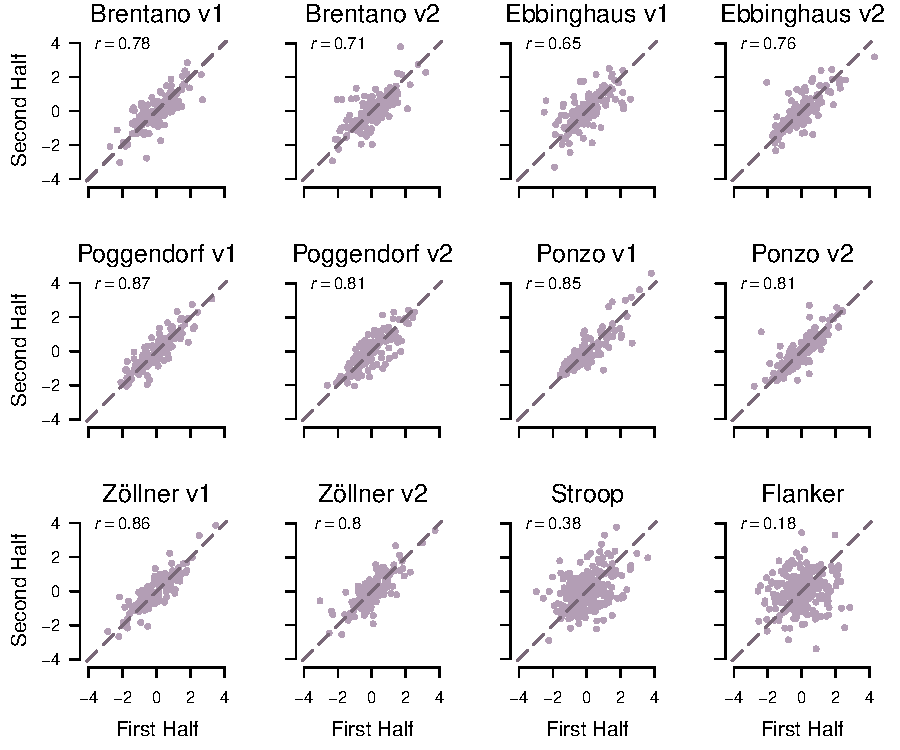
\includegraphics[width=6in, height=5in]{_figs/split-halves.pdf}
    \caption{Split-half reliabilities serve as check.  Even though the halves may differ systematically from learning and are comprised of 7 and 8 trials, respectively, the reliability is high.  Split-half reliability for cognitive control is less even though there are over 10X as many trials, and this result again highlights the lack of trial noise in illusion tasks compared to cognitive control tasks.}
    \label{fig:relPlots}
\end{figure}


\begin{figure}
    \centering  % Centers the figure
    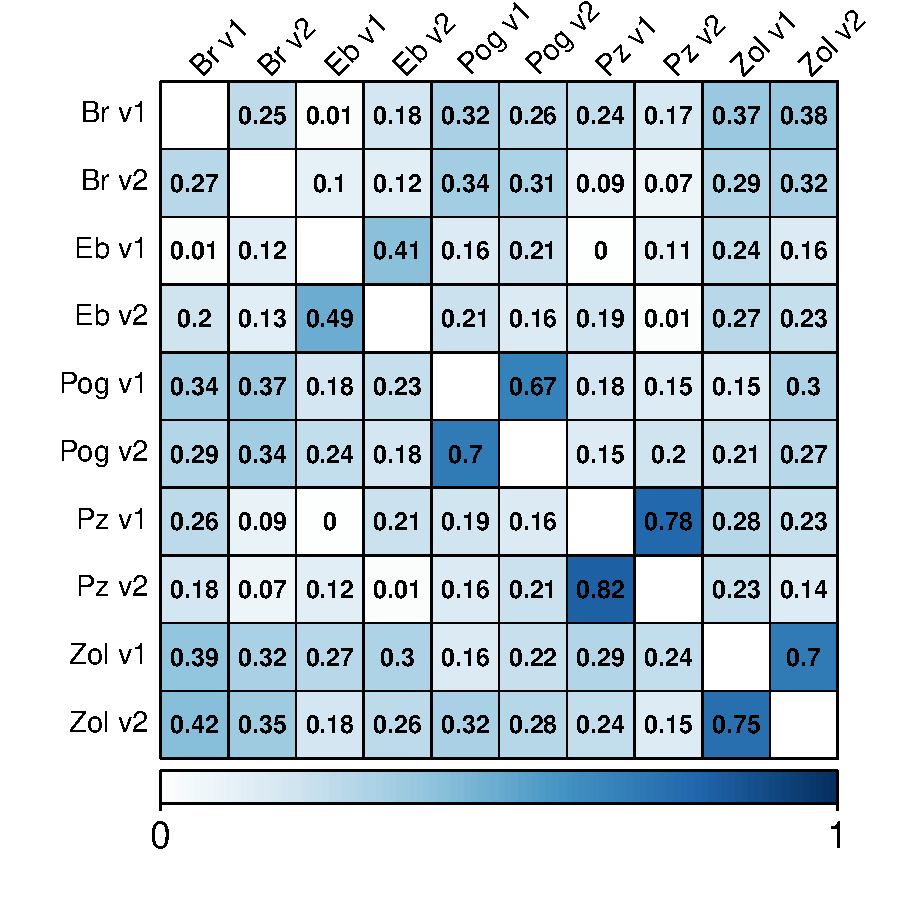
\includegraphics[width=6in, height=6in]{_figs/cor.pdf}
    \caption{Correlations across tasks.  The upper triangle shows sample correlations.  The lower triangle is model-estimated correlations from the hierarchical Wishart model.   Sample and model correlations are quite close reflecting a low degree of trial noise.  The defining features are large correlations between versions for the Poggendorf, Ponzo, and Zöllner Illusions, but more marginal correlations for Brentano and Ebbinghaus Illusions.}
    \label{fig:corPlot}
\end{figure}


\begin{figure}
    \centering  % Centers the figure
    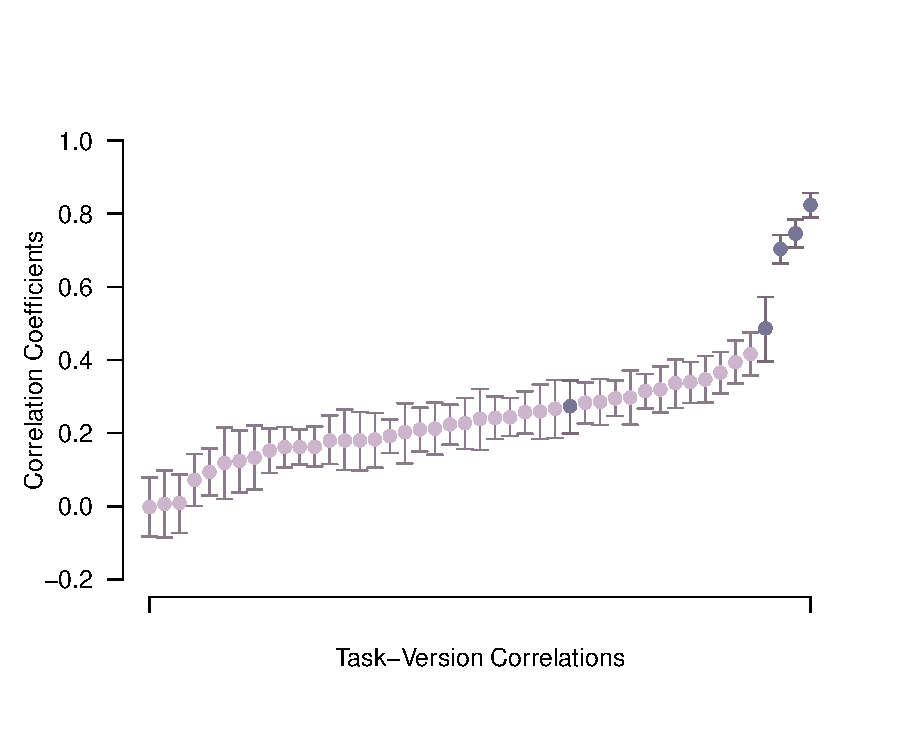
\includegraphics[width=6in, height=5in]{_figs/cor-CI.pdf}
    \caption{Uncertainties in correlations.  Shown are model correlations (lower triangle in Figure 5) along with 95\% credible intervals.  The three version correlations are well separated; the cross-task correlations center around .22 in value.}
    \label{fig:ciCorPlots}
\end{figure}


\begin{figure}
    \centering  % Centers the figure
    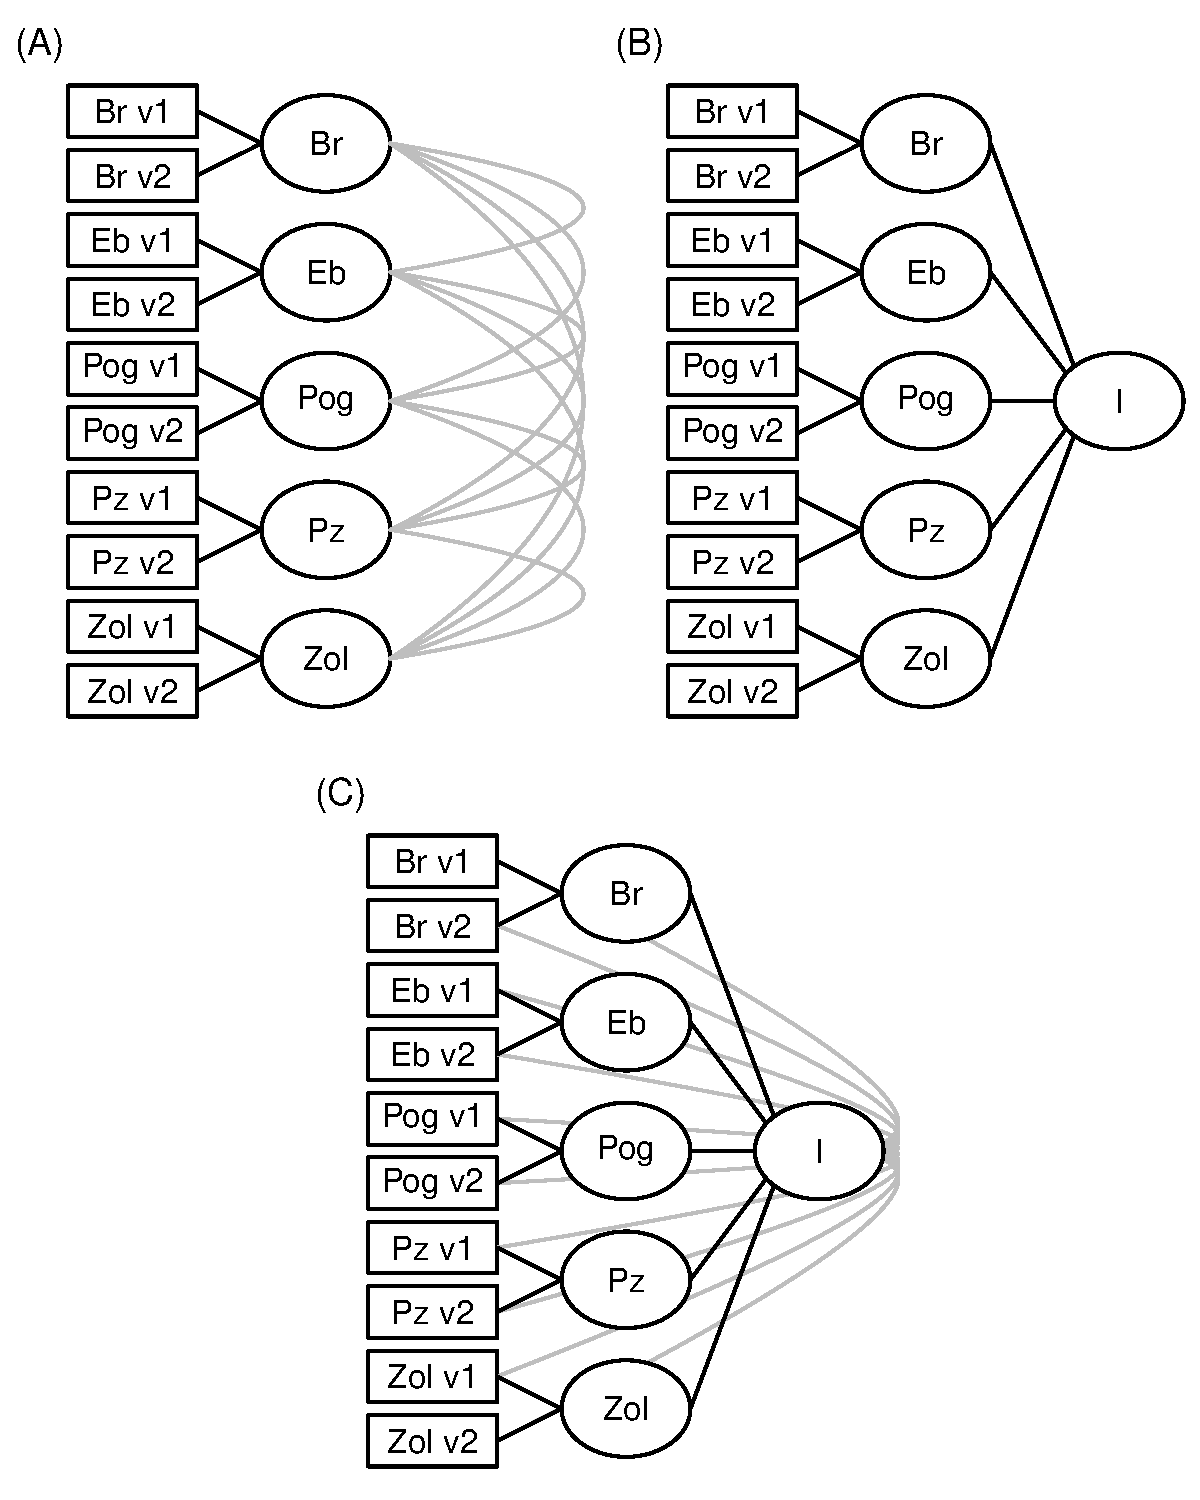
\includegraphics[width=6in, height=8in]{_figs/factor_cfa.pdf}
    \caption{Three confirmatory factor models did not yield interpretable results.}
    \label{fig:cfa}
\end{figure}

\begin{table}[htbp]
    \centering
    \caption{Exploratory Factor Analysis Model Selection Statistics.}
    \label{tab:EFA-10}
    \begin{threeparttable}
        \begin{tabular}{cccccc
        }
            \toprule
            {# Factors} & {PCA Eigenvalue} & {AIC} & {BIC} & {CFI} & {RMSEA}\\
            \midrule
            1 & 3.239 & 3734.880 & 3793.425 & 0.463 & 0.220\\
            2 & 1.545 & 3630.132 & 3715.022 & 0.724 & 0.183\\
            3 & 1.261 & 3554.424 & {\textbf{3662.733}} & 0.917 & 0.121\\
            4 & \textbf{1.183} & 3537.297 & 3666.097 & 0.972 & 0.089\\
            5 & 0.771 & {\textbf{3527.484}} & 3673.847 & 1.000 & 0.000\\
            6 & 0.682 & 3536.200 & 3697.198 & 1.000 & 0.000\\
            \bottomrule
        \end{tabular}
        \vspace{5pt}
        \begin{tablenotes}
            \small
            \item Note: Boldface typeset indicates number of selected factors.  These are 4 by eigenvalues, 5 by AIC and 3 by BIC.
        \end{tablenotes}
    \end{threeparttable}
\end{table}


\begin{table}[htbp]
    \centering
    \caption{Exploratory Factor Analysis Loadings}
    \label{tab:Fac-10}
    \begin{threeparttable}
        \begin{tabular}{l|ccccc|cc}
            \toprule
            Task-Version
            & \multicolumn{5}{c|}{Factor Loadings} & \multicolumn{2}{c}{Proportion of Variance} \\
            \cmidrule{2-8}
             & 1 & 2 & 3 & 4 & 5 & Unique & Shared \\
            \midrule
            Brentano v1 & \textit{0.401} & 0.145 & \textit{0.279} & 0.124 & -0.119 & 0.711 & 0.289 \\
            Brentano v2 & \textit{0.315} & 0.008 & \textit{0.336} & 0.019 & 0.041 & 0.785 & 0.215 \\
            Ebbinghaus v1 & 0.096 & 0.014 & 0.124 & 0.223 & \textbf{0.724} & 0.401 & 0.599 \\
            Ebbinghaus v2 & 0.163 & 0.043 & 0.103 & \textbf{0.854} & 0.267 & 0.160 & 0.840 \\
            Poggendorf v1 & 0.119 & 0.072 & \textbf{0.904} & 0.104 & 0.013 & 0.152 & 0.848 \\
            Poggendorf v2 & 0.154 & 0.101 & \textbf{0.704} & 0.021 & 0.155 & 0.446 & 0.554 \\
            Ponzo v1 & 0.189 & \textbf{0.811} & 0.092 & 0.175 & -0.115 & 0.254 & 0.746 \\
            Ponzo v2 & 0.072 & \textbf{0.976} & 0.094 & -0.113 & 0.144 & 0.000 & 1.000 \\
            Zoellner v1 & \textbf{0.870} & 0.147 & 0.034 & 0.080 & 0.181 & 0.182 & 0.818 \\
            Zoellner v2 & \textbf{0.771} & 0.070 & 0.209 & 0.081 & 0.049 & 0.348 & 0.652 \\
            \bottomrule
        \end{tabular}
        \vspace{5pt}
        \begin{tablenotes}
            \small
            \item Note. Boldfaced loadings highlight the relations between factors and tasks.
        \end{tablenotes}
    \end{threeparttable}
\end{table}

\begin{table}[htbp]
    \centering
    \caption{Exploratory Factor Analysis Model Selection Statistics When Certain Versions Are Removed}
    \label{tab:EFA-5}
    \begin{threeparttable}
        \begin{tabular}{cccccc}
            \hline
            \ {Factors} & {PCA Eigenvalue} & {AIC} & {BIC} & {CFI} & {RMSEA} \\
            \hline
            1 & \textbf{1.967} & \textbf{1911.33} & \textbf{1940.6} & 0.99 & 0.03\\
            2 & 0.877 & 1914.3 & 1955.28 & 1
            & 0.00\\
            \hline
        \end{tabular}
        \vspace{5pt}
        \begin{tablenotes}
            \small
            \item Note: Boldfaced items show selected models.  All methods lead to a one-factor model.
        \end{tablenotes}
    \end{threeparttable}
\end{table}


\begin{table}[htbp]
    \centering
    \caption{Exploratory Factor Analysis Model Loadings When Certain Versions Are Removed}
    \label{tab:Fac-5}
    \begin{threeparttable}
        \begin{tabular}{l|c|cc}
            \toprule
            Task-Version
            & \multicolumn{1}{c|}{Factor Loadings} & \multicolumn{2}{c}{Proportion of Variance} \\
             &  & Unique & Shared \\
            \midrule
            Brentano v1 & 0.606 & 
            0.633 & 0.367 \\
            Ebbinghaus v2 & 0.400 & 
            0.840 & 0.160 \\
            Poggendorf v1 & 0.421 & 
            0.823 & 0.177 \\
            Ponzo v1 & 0.445 & 
            0.802 & 0.198 \\
            Zoellner v1 & 0.578 & 
            0.666 & 0.334 \\
            \bottomrule
        \end{tabular}
        \vspace{5pt}
    \end{threeparttable}
\end{table}


\end{document}